\documentclass[a4paper,11pt]{scrartcl}
\usepackage[utf8x]{inputenc}
\usepackage[catalan]{babel}
\usepackage{titlesec}
% A ses llengües llatines, el primer paràgraf ha d'anar tabulat
\usepackage{indentfirst}
\usepackage{amsmath}
\usepackage{float}
\usepackage{graphicx}
\usepackage{subfigure}
\usepackage{booktabs}
\usepackage{multirow}
\usepackage{hyperref}
\usepackage{url}
\usepackage{multirow}
\usepackage{minted} %wget http://minted.googlecode.com/hg/minted.sty

% aptitude install texlive-fonts-extra
\usepackage{newcent} %font mes wapa

\graphicspath{{diagrames/}}

% Estil de seccions
\titleformat{\section}{\large\sectfont}{\thesection}{1em}{}
\titleformat{\subsection}{\bfseries\sectfont}{\thesubsection}{1em}{}
% Estil numeracio subseccions http://help-csli.stanford.edu/tex/latex-sections.shtml#number
%\def\thesubsection{\alph{subsection})}

\title{Robòtica: \\ Rainer\footnote{Explicació de que vol dir rainer} \ Project}
\author{ Bartomeu Miró Mateu \thanks{bartomeumiro a gmail punt com} \\
	 Lluis Cortès Rullan \thanks{lluisbinet a gmail punt com} }

\begin{document}

  \maketitle

  \begin{abstract}
    Segona pràctica de Robòtica emmarcada a l'apartat de robòtica mòbil.
    Programació d'una arquitectura de control per un robot Pioneer-3DX que
    permeti moure’s per un entorn amb obstacles i netejar un area mapejant
    els obstacles.
  \end{abstract}

  \newpage
  \setcounter{page}{2}
  \tableofcontents
  \newpage

  \section{Interpretació de l'enunciat}

En l'enunciat es descriu essencialment com dur a terme l'evitació d'obstacles i finalment
es proposen una sèrie de tasques a implementar com ara recorrer un conjunt de punts, vagar etc.

En aquesta pràctica s'implementa un robot netejador que vendria a ser un eufemisme per dir un
robot que intenta cobrir tots els punts d'una determinada àrea evitant els obstacles.

A banda d'aquesta funció principal també s'ha implementat la funcionalitat de vagar.

En aquesta implementació no es destaca l'originalitat de l'acció duita a terme (robot de neteja)
sinó que s'ha intentat fer èmfasi em la jerarquia de l'arquitectura i l'encapsulat de les funcions de tal
manera que un cop establert això és molt senzill desenvolupar noves tasques o afegir i modificar
funcionalitats, tema que es torna a tractar en l'apartat de possibles ampliacions.
  \include{modelitzacio}
  \include{implementacio} %%inclou funcionalitat
  \include{limitacionsIproblematica}
  \section{Joc de proves}

Per tal de provar la pràctica s'han realitzat una sèrie de jocs de proves
descrits a continuació. Per cada un d'ells s'ha generat un mapa amb el
\emph{Mapper3Basic} i es poden trobar a la carpeta \emph{maps}.

Al \texttt{Makefile} es troben totes les opcions comentades a l'apartat \emph{sim}, així doncs
es descomenta la desitjada i es comenta la que està per defecte. A continuació
es canvia el codi font
de \texttt{rainer.cpp} comentant el cleanArea i descomentant l'opció desitjada.
Un cop fet això amb un \emph{make} és compila el codi i amb el \emph{make sim}
s'executa el simulador.

El primer test és simple, \textbf{passar per quatre punts sense cap obstacle}. Amb aquest simplement es comprova que es calculi
bé el vector d'atracció. També es pot observar si el \emph{heading} es fa de
manera adequada. Per fer aquesta execució no s'empre cap mapa.

\begin{figure}[H]
\begin{center}\label{4punts}
 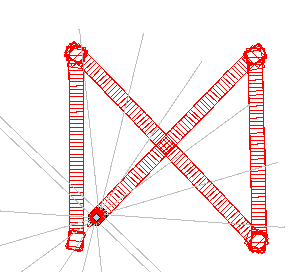
\includegraphics[width=0.5\textwidth]{diagrames/figures/4punts.png}
 % ordreRotacions.png: 1286x768 pixel, 150dpi, 21.77x13.00 cm, bb=0 0 617 369
\end{center}
  \caption{Quatre puts sense obstacle}
\end{figure}

En segon lloc tenim \textbf{passar per quatre punts però amb un obstacle}
enmig. En aquest es veu si l'esquiva d'obstacles es fa bé. A més l'obstacle està
co\lgem ocat de tal manera que el robot es troba impactant una línia de 45 graus
amb el punt destí a la perpendicular, de tal manera que seria una situació
delicada on quedar-se estancat. Per fer aquesta execució s'empra el mapa
\emph{obstacleInclinat}.

\begin{figure}[H]
\begin{center}\label{4puntsObs}
 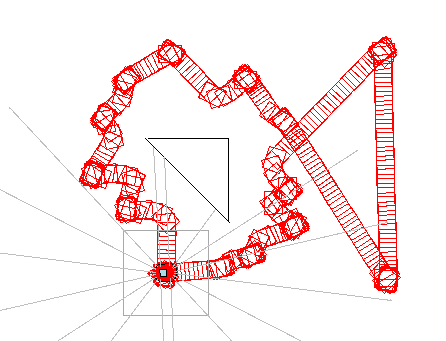
\includegraphics[width=0.5\textwidth]{diagrames/figures/4puntsObs.png}
 % ordreRotacions.png: 1286x768 pixel, 150dpi, 21.77x13.00 cm, bb=0 0 617 369
\end{center}
  \caption{Quatre puts sense obstacle}
\end{figure}

A continuació trobam el mateix \textbf{obstacle} però aquest cop \textbf{situat sobre el punt de destí}, en aquest cas
el robot ha de detectar que no pot arribar-hi ja que l'obstacle i el punt de
destí estan per davall d'un cert llindar. Fins que no s'assoleix aquest llindar
es veu com el robot intenta fer aproximacions al punt desde diferents
direccions. En aquest test empram el mapa \emph{obstacleApunt}.

\begin{figure}[H]
\begin{center}\label{obsapunt}
 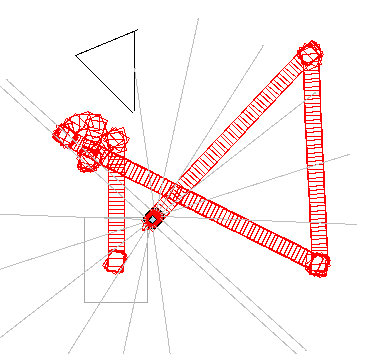
\includegraphics[width=0.5\textwidth]{diagrames/figures/obsapunt.png}
 % ordreRotacions.png: 1286x768 pixel, 150dpi, 21.77x13.00 cm, bb=0 0 617 369
\end{center}
  \caption{Quatre puts sense obstacle}
\end{figure}

Per tal de provar el \textbf{vagar} tenim un mapa tancat amb diversos obstacles
on el robot va rebotant.
Pot arribar un punt en que el robot entri en un cicle ja que els angles de rebot
poden fer que així coincideixi. El que no es permet es que el robot toqui un
obstacle o es quedi immòbil sols girant sobre ell mateix sense ser capaç de
emprendre la ruta cap a una altra banda.

\begin{figure}[H]
\begin{center}\label{vagant}
 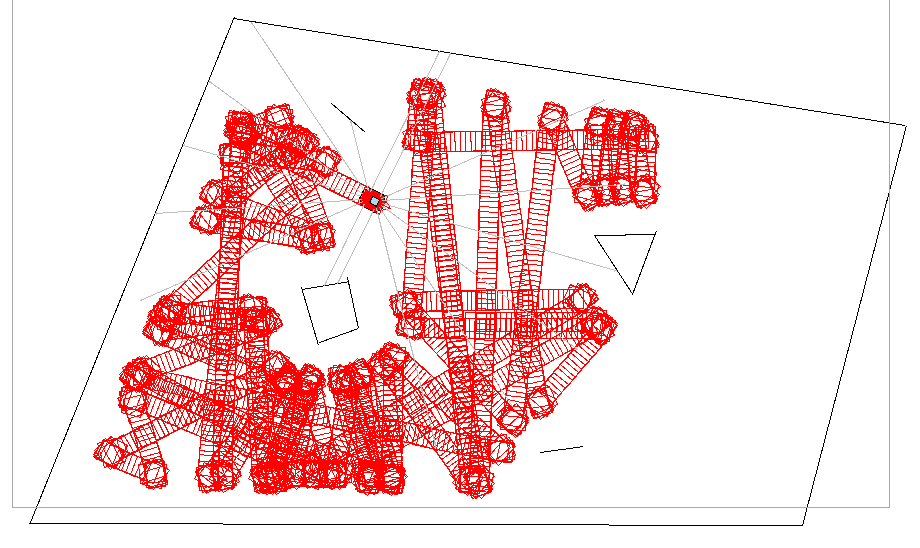
\includegraphics[width=0.5\textwidth]{diagrames/figures/vagant.png}
 % ordreRotacions.png: 1286x768 pixel, 150dpi, 21.77x13.00 cm, bb=0 0 617 369
\end{center}
  \caption{Quatre puts sense obstacle}
\end{figure}

A continuació tenim les proves de la \textbf{neteja de zona}, la primera \textbf{sense obstacles} per veure el recorregut.

\begin{figure}[H]
\begin{center}\label{neteja}
 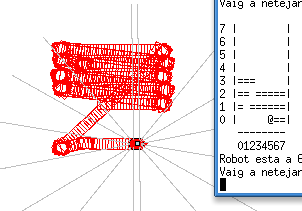
\includegraphics[width=0.5\textwidth]{diagrames/figures/netNoObs.png}
 % ordreRotacions.png: 1286x768 pixel, 150dpi, 21.77x13.00 cm, bb=0 0 617 369
\end{center}
  \caption{Quatre puts sense obstacle}
\end{figure}

I finalment la \textbf{neteja amb obstacles} on el robot els esquiva (i marca terreny durant aquesta esquiva)
i com finalment torna a les zones d'obstacle per comprovar que no fos un
obstacle mòbil i ara si que pot netejar la zona. En aquest últim no podem
simular obstacles mòbils però si veure com torna a intentar anar a la zona
obstaculitzada.

\begin{figure}[H]
\begin{center}\label{netejaobs}
 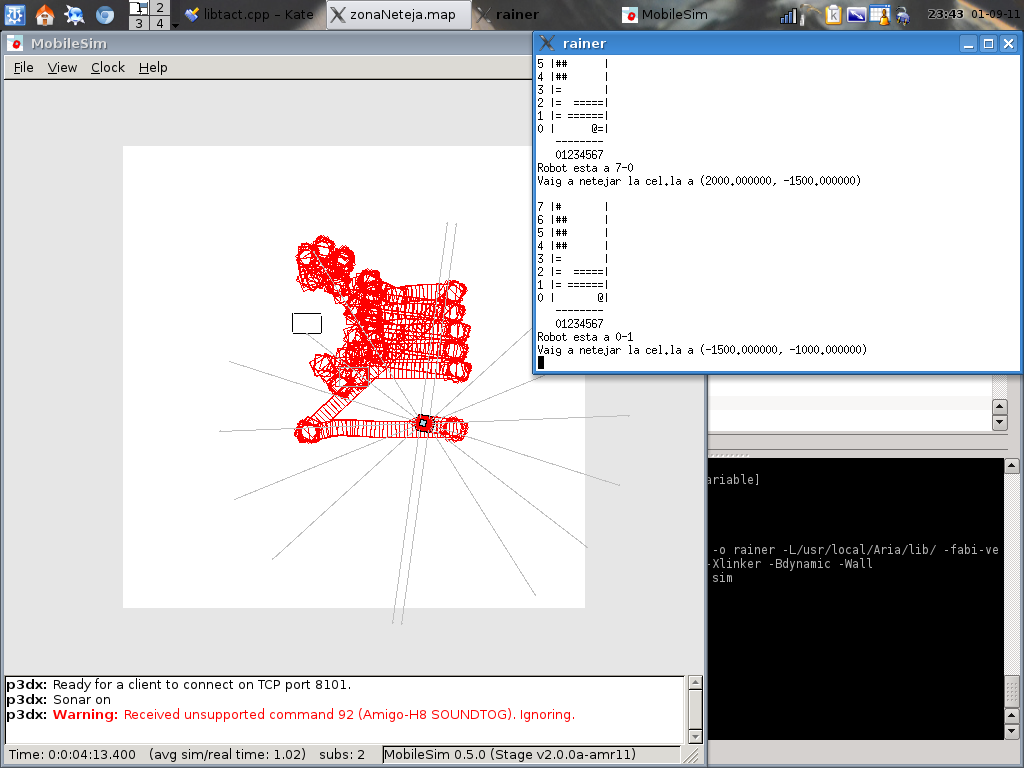
\includegraphics[width=0.5\textwidth]{diagrames/figures/netejant.png}
 % ordreRotacions.png: 1286x768 pixel, 150dpi, 21.77x13.00 cm, bb=0 0 617 369
\end{center}
  \caption{Primera passada de la neteja}
\end{figure}

\begin{figure}[H]
\begin{center}\label{figescenari}
 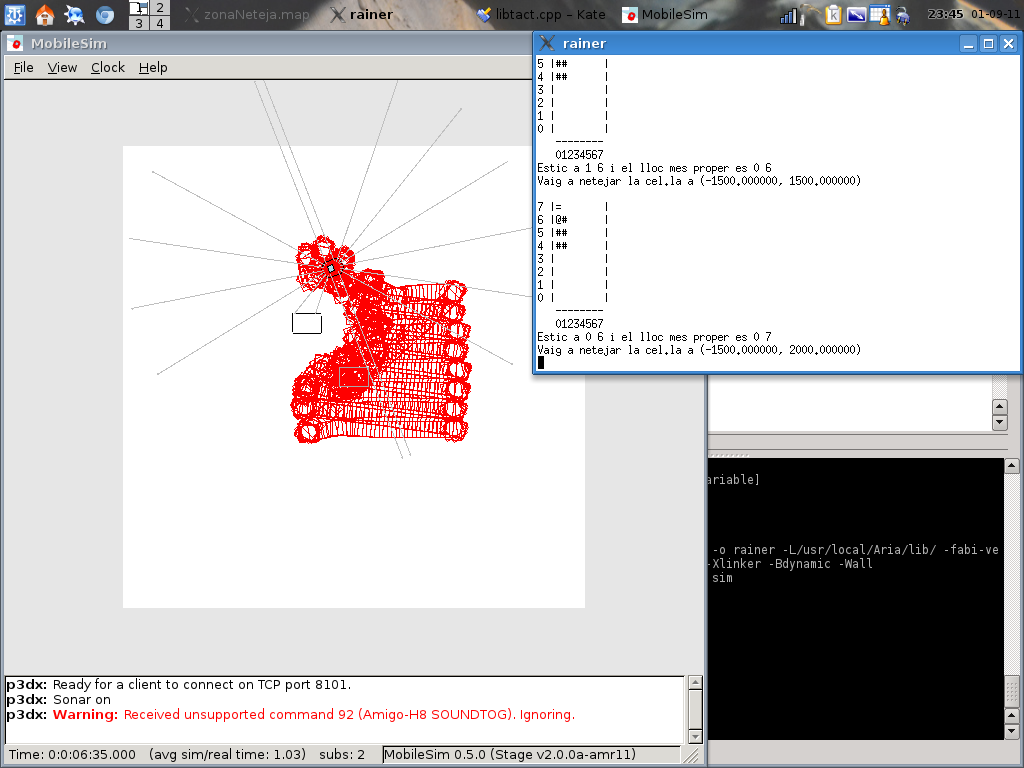
\includegraphics[width=0.5\textwidth]{diagrames/figures/netejant-aobstacles.png}
 % ordreRotacions.png: 1286x768 pixel, 150dpi, 21.77x13.00 cm, bb=0 0 617 369
\end{center}
  \caption{Segona passada de la neteja anant als punts detectats com obstacle}
\end{figure}


  \section{Possibles ampliacions}

En aquest apartat es mencionen possibles ampliacions de la pràctica actual. El fet de fer aquestes mencions
és perquè així es demostra la flexibilitat de l'arquitectura implementada i alhora mostra el grau
de comprensió adquirit veient com es podria continuar treballant.

El fet de no implementar aquestes ampliacions es perquè és costós en temps per els pocs coneixements
que es demostren.

\subsection{Ruta de neteja òptima}
Una primera millora seria implementar un viatjant de comerç per passar a fer la neteja de tots els punts.
Per fer això simplement seria necessari implementar la funció que generés la ruta òptima, guardar-la en 
memòria i implementar un iterador perquè cada crida de la funció \texttt{getNextCell} recorrér el punt on s'ha d'anar.
Dit iterador es una simple vector amb un punter també conegut com \emph{array vulgaris}.
Amb aquesta implementació s'evitarien recorregunts innecessaris sobre ce\lgem es ja netejades i el recorregut
mínim per fer-ho.

Hem de tenir amb compte que el cost és NP i el fet de trobar un obstacle pot esgarrar fàcilment la ruta.

\subsection{Atenció d'emergències}
Per altra banda seria senzill implementar una espera d'esdeveniments de teclat perquè el robot atengui una urgència,
simplement podria fer-se amb una tasca nova pendent d'esdeveniments de teclat que sobreescrigui el valor del  punt
on ha d'anar el robot.

Notem que com que la tasca de posicionar el robot al mapa i de mirar que s'ha netejat són una tasca apartat
a l'atendre una emergència també es considerarien nets els punts per on ha passat per atendre-la.

\subsection{Inaccessibilitat}
Finalment també es podria treballar el fet de trobar llocs inaccessibles. Una opció per fer-ho
es un cop iniciat el moviment a un punt guardar en un vector els punts per on es passa i quan passa
cert llindar de temps mirar si la posició actual es un punt ja dins del vector, així podríem comprovar
si està movent-se de costat a costat intentant accedir a un lloc on no es possible.

Dita funcionalitat sol requereix una lleu modificació a la tasca que registra els punts per on s'està
passat i una variable de comunicació.

\subsection{Imatge del mapa}

Finalment també seria interessant que la tasca que vigila el valors dels sensors escrivís a un mapa de bits
les lectures fetes, així es tindria una imatge amb el mapa de la situació. Aquesta funcionalitat 
en l'estat actual de la pràctica és molt senzilla de implementar, però requereix tenir soltura emprant
mapes de bits i generant imatges.

A l'igual que l'anterior seria una modificació a la tasca que registra els punts per on s'està passant.
  \emph{Valoració}

La practica ha resultat molt interessant, al principi va costar un poc adequar l'entorn de treball.
Per tal de poder emprar la llibreria i el simulador \emph{MobileSim} en la \emph{Debian} que empram normalment
va requerir compilar-ho de nou cosa que generà algun problema de dependències però va quedar sobradament
compensat per la comoditat de no haver de emprar una màquina virtual.

Cal destacar que el \emph{Mapper3Basic} i el \emph{MobileSim} són de gran ajuda a l'alumne i permeten fer simulacions
per res comparables amb la primera pràctica del braç robot que resulten vitals per el desenvolupament de la pràctica.

La llibreria \emph{Aria} en general esta força bé i és bastant intuïtiva, rara vegada s'ha hagut de cercar
informació addicional que no figurés a la API.

Per altra banda s'ha de mencionar que el \emph{C++} ens ha suposat algun mal de cap, sobretot en l'àmbit
de visibilitat dels procediments i l'ús de punters. En aquest sentit ens hagués agradat tenir temps
per provar de fer la pràctica amb \emph{Python} ja que l'\emph{Aria} en te uns \emph{bindings}. 
L'únic fet que ens tirà endarrere es que no sabíem si funcionaria
el simulador i que possiblement la llibreria no està insta\lgem al robot real.

També ens han portat molts mal de cap el trobar valors adequats per cada una de les ponderacions i llindars,
sovint ens trobàvem que amb certa combinació de llindars, especialment als de \emph{heading} el robot podia quedar
fent voltes sobre si mateix si el punt on havia d'anar era proper al punt actual però havia de fer un canvi
d'orientació. 

\begin{figure}[H]
\begin{center}\label{headingthproblem}
 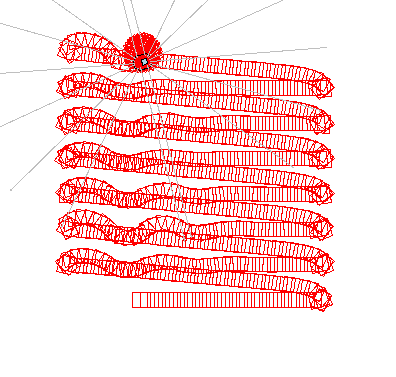
\includegraphics[width=0.5\textwidth]{diagrames/figures/voltes.png}
 % ordreRotacions.png: 1286x768 pixel, 150dpi, 21.77x13.00 cm, bb=0 0 617 369
\end{center}
  \caption{Problema amb llindar de heading}
\end{figure}

Atribuirem aquest problema a que el robot inicia el moviment abans d'estar orientat però donat que la
proximitat es molt gran no acaba d'orientar-se mai.


Tot i així i encara que ens hagués agradat implementar alguna cosa més consideram la pràctica acabada
i assolits els coneixements bàsics i que per tant les implementacions que tenim en ment i figuren en l'apartat
d'ampliacions es converteien en rutina ja que no requereixen conceptes nous sinó simples combinacions i modificacions 
sobre l'arquitectura i rutines ja implementats. %% De la practica i tecnologia emprara en si i tamb e de contingut
  \section{Annex: Codi font complet}

\subsection{Rainer, cos principal}
\inputminted[linenos, frame=lines, fontsize=\footnotesize]{cpp}{../rainer.cpp}
\newpage
\subsection{librainer, llibreria de l'estratègic}
\inputminted[linenos, frame=lines, fontsize=\footnotesize]{cpp}{../librainer.h}
\inputminted[linenos, frame=lines, fontsize=\footnotesize]{cpp}{../librainer.cpp}
\newpage
\subsection{libtact, llibreria del nivell tàctic}
\inputminted[linenos, frame=lines, fontsize=\footnotesize]{cpp}{../libtact.h}
\inputminted[linenos, frame=lines, fontsize=\footnotesize]{cpp}{../libtact.cpp}
\newpage
\subsection{librainermap, llibreria transversal del mapa}
\inputminted[linenos, frame=lines, fontsize=\footnotesize]{cpp}{../librainermap.h}
\inputminted[linenos, frame=lines, fontsize=\footnotesize]{cpp}{../librainermap.cpp}
\newpage
\subsection{lib2d, llibreria transversal d'aritmètica de vectors i punts}
\inputminted[linenos, frame=lines, fontsize=\footnotesize]{cpp}{../lib2d.h}
\inputminted[linenos, frame=lines, fontsize=\footnotesize]{cpp}{../lib2d.cpp}

\end{document}
